%%
%% This is file `sample-sigconf.tex',
%% generated with the docstrip utility.
%%
%% The original source files were:
%%
%% samples.dtx  (with options: `sigconf')
%% 
%% IMPORTANT NOTICE:
%% 
%% For the copyright see the source file.
%% 
%% Any modified versions of this file must be renamed
%% with new filenames distinct from sample-sigconf.tex.
%% 
%% For distribution of the original source see the terms
%% for copying and modification in the file samples.dtx.
%% 
%% This generated file may be distributed as long as the
%% original source files, as listed above, are part of the
%% same distribution. (The sources need not necessarily be
%% in the same archive or directory.)
%%
%% Commands for TeXCount
%TC:macro \cite [option:text,text]
%TC:macro \citep [option:text,text]
%TC:macro \citet [option:text,text]
%TC:envir table 0 1
%TC:envir table* 0 1
%TC:envir tabular [ignore] word
%TC:envir displaymath 0 word
%TC:envir math 0 word
%TC:envir comment 0 0
%%
%%
%% The first command in your LaTeX source must be the \documentclass command.
% \documentclass[sigconf]{acmart}


\documentclass[sigconf,review,anonymous]{acmart}
% \documentclass[sigconf,review]{acmart}

%% NOTE that a single column version may be required for 
%% submission and peer review. This can be done by changing
%% the \doucmentclass[...]{acmart} in this template to 
%% \documentclass[manuscript,screen]{acmart}
%% 
%% To ensure 100% compatibility, please check the white list of
%% approved LaTeX packages to be used with the Master Article Template at
%% https://www.acm.org/publications/taps/whitelist-of-latex-packages 
%% before creating your document. The white list page provides 
%% information on how to submit additional LaTeX packages for 
%% review and adoption.
%% Fonts used in the template cannot be substituted; margin 
%% adjustments are not allowed.
%%
%%
%% \BibTeX command to typeset BibTeX logo in the docs
\AtBeginDocument{%
  \providecommand\BibTeX{{%
    \normalfont B\kern-0.5em{\scshape i\kern-0.25em b}\kern-0.8em\TeX}}}

%% Rights management information.  This information is sent to you
%% when you complete the rights form.  These commands have SAMPLE
%% values in them; it is your responsibility as an author to replace
%% the commands and values with those provided to you when you
%% complete the rights form.

\setcopyright{acmcopyright}
\copyrightyear{2024}
\acmYear{2024}
\acmDOI{XXXXXXX.XXXXXXX}

\settopmatter{printacmref=true} %remove ACM reference format

% %% These commands are for a PROCEEDINGS abstract or paper.
% \acmConference[Conference acronym 'XX]{Make sure to enter the correct
%   conference title from your rights confirmation emai}{June 03--05,
%   2018}{Woodstock, NY}

\acmConference[CF 24]{The 21st ACM International Conference on Computing Frontiers}{May 2024}{Ischia, Naples, Italy}

% %
% %  Uncomment \acmBooktitle if th title of the proceedings is different
% %  from ``Proceedings of ...''!
% %
% %\acmBooktitle{Woodstock '18: ACM Symposium on Neural Gaze Detection,
% %  June 03--05, 2018, Woodstock, NY} 
\acmPrice{15.00}
\acmISBN{978-1-4503-XXXX-X/18/06}


%%
%% Submission ID.
%% Use this when submitting an article to a sponsored event. You'll
%% receive a unique submission ID from the organizers
%% of the event, and this ID should be used as the parameter to this command.
\acmSubmissionID{28}

%%
%% For managing citations, it is recommended to use bibliography
%% files in BibTeX format.
%%
%% You can then either use BibTeX with the ACM-Reference-Format style,
%% or BibLaTeX with the acmnumeric or acmauthoryear sytles, that include
%% support for advanced citation of software artefact from the
%% biblatex-software package, also separately available on CTAN.
%%
%% Look at the sample-*-biblatex.tex files for templates showcasing
%% the biblatex styles.
%%

%%
%% The majority of ACM publications use numbered citations and
%% references.  The command \citestyle{authoryear} switches to the
%% "author year" style.
%%
%% If you are preparing content for an event
%% sponsored by ACM SIGGRAPH, you must use the "author year" style of
%% citations and references.
%% Uncommenting
%% the next command will enable that style.
%% \citestyle{acmauthoryear}

\usepackage{makecell}
\usepackage{listings}
\usepackage{subcaption}
\usepackage{float}
\usepackage{multirow}
\usepackage{multicol}
\usepackage{enumitem}

\usepackage{fancyhdr}
\pagestyle{empty}

\usepackage{minted}
\usepackage{mdframed}
\usepackage{booktabs}

\usepackage{algorithm}
\usepackage{algorithmicx}
\usepackage{algpseudocode}

%%
%% end of the preamble, start of the body of the document source.
\begin{document}

%%
%% The "title" command has an optional parameter,
%% allowing the author to define a "short title" to be used in page headers.
\title{COPS: A coroutine-based priority scheduling framework perceived by the operating system}

%%
%% The "author" command and its associated commands are used to define
%% the authors and their affiliations.
%% Of note is the shared affiliation of the first two authors, and the
%% "authornote" and "authornotemark" commands
%% used to denote shared contribution to the research.
\author{Fangliang Zhao}
\affiliation{%
  \institution{Tsinghua University}
  \streetaddress{30 Shuangqing Rd}
  \city{Haidian Qu}
  \state{Beijing Shi}
  \country{China}
}
\email{zfl22@mails.tsinghua.edu.cn}
\orcid{0009-0001-3860-6011}

\author{Donghai Liao}
\affiliation{%
  \institution{Beijing Institute of Technology}
  \streetaddress{No. 5 Zhongguancun South Street}
  \city{Haidian Qu}
  \state{Beijing Shi}
  \country{China}
}
\email{ctrlz.donghai@gmail.com}

\author{Jingbang Wu}
\affiliation{%
  \institution{Beijing Technology and Business University}
  \city{Haidian Qu}
  \state{Beijing Shi}
  \country{China}
}
\email{wujingbang@btbu.edu.cn}
\orcid{0000-0002-1394-5631}

\author{Huimei Lu}
\affiliation{%
  \institution{Beijing Institute of Technology}
  \streetaddress{No. 5 Zhongguancun South Street}
  \city{Haidian Qu}
  \state{Beijing Shi}
  \country{China}
}
\email{luhuimei@bit.edu.cn}

\author{Yong Xiang}
\affiliation{%
  \institution{Tsinghua University}
  \streetaddress{30 Shuangqing Rd}
  \city{Haidian Qu}
  \state{Beijing Shi}
  \country{China}
}
\email{xyong@tsinghua.edu.cn}
\orcid{0000-0003-1092-2183}

%%
%% By default, the full list of authors will be used in the page
%% headers. Often, this list is too long, and will overlap
%% other information printed in the page headers. This command allows
%% the author to define a more concise list
%% of authors' names for this purpose.
% \renewcommand{\shortauthors}{Trovato and Tobin, et al.}

%%
%% The abstract is a short summary of the work to be presented in the
%% article.
\begin{abstract}

The multi-threading model in the general operating systems is becoming insufficient in applications with increasing amounts of concurrency, due to the context-switching costs in the kernel multi-threading. In this paper, a new concurrency model named COPS is proposed. COPS uses a priority-based coroutine model as the smallest task unit to replace the multi-threading model in large concurrency scenarios, and provides a unified priority-based scheduling framework for kernel space and user space coroutines. COPS introduces coroutines as first-class objects in the OS to provide asynchronous I/O mechanism, which takes kernel coroutines as a bridge between I/O operations and devices and takes user coroutines as a bridge between applications and the OS's services respectively.

We design a prototype of web server based on COPS and conduct extensive experiments in an FPGA-based system to evaluate COPS. Results show that the proposed model achieves one to four times higher throughput while remains relatively lower overhead than that using the multi-threading model in the large concurrency applications.

\end{abstract}

%%
%% The code below is generated by the tool at http://dl.acm.org/ccs.cfm.
%% Please copy and paste the code instead of the example below.
%%
\begin{CCSXML}
<ccs2012>
   <concept>
       <concept_id>10011007.10010940.10010941.10010949.10010957.10010688</concept_id>
       <concept_desc>Software and its engineering~Scheduling</concept_desc>
       <concept_significance>500</concept_significance>
       </concept>
   <concept>
       <concept_id>10011007.10010940.10010941.10010949.10010957.10010959</concept_id>
       <concept_desc>Software and its engineering~Multiprocessing / multiprogramming / multitasking</concept_desc>
       <concept_significance>500</concept_significance>
       </concept>
 </ccs2012>
\end{CCSXML}

\ccsdesc[500]{Software and its engineering~Scheduling}
\ccsdesc[500]{Software and its engineering~Multiprocessing / multiprogramming / multitasking}

%%
%% Keywords. The author(s) should pick words that accurately describe
%% the work being presented. Separate the keywords with commas.
\keywords{Multi-threading, Concurrency, Coroutine.}

%% A "teaser" image appears between the author and affiliation
%% information and the body of the document, and typically spans the
%% page.
% \begin{teaserfigure}
%   \includegraphics[width=\textwidth]{sampleteaser}
%   \caption{Seattle Mariners at Spring Training, 2010.}
%   \Description{Enjoying the baseball game from the third-base
%   seats. Ichiro Suzuki preparing to bat.}
%   \label{fig:teaser}
% \end{teaserfigure}

% \received{20 February 2007}
% \received[revised]{12 March 2009}
% \received[accepted]{5 June 2009}

%%
%% This command processes the author and affiliation and title
%% information and builds the first part of the formatted document.
\maketitle

\section{Introduction}
\label{section: introduction}

In today's era of data explosion, the ability of the general Operating Systems (OS) to process large amounts of data is receiving more attention. For example, Google's servers handle 883 billion requests per day in 2022 \cite{google-search-statistics}, with an average of 8 million requests per second. The increasing scale of the concurrency in the system poses severe challenges to the traditional multi-threading model, which has two main shortcomings in our point of view. First, the multi-threading model is nondeterministic \cite{Lee:EECS-2006-1}. The execution order of threads is uncertain, resulting in the access order of shared resources being uncertain. When used inappropriately in fixed workflows, multi-threading can lead to greater overhead. In order to improve the performance of the multi-threading model in large concurrency scenarios such as the web server, some research has tried to optimize it, but has not solved the problem mechanically \cite{li_combining_2007, howell_cooperative_2002}.

Second, the multi-threading model is incompatible with the asynchronous I/O mechanism in OS. The traditional OS such as Linux usually utilizes the event-driven model to achieve the asynchronous I/Os, resulting in the complexity of OS. For example, Linux provides system calls such as the select and epoll to support user-level asynchronous I/O tasks by reusing multiple I/O operations on a single thread \cite{Gammo2004ComparingAE}. The epoll process combines a single thread with an event-driven model, and requires interaction through the producer-consumer model, which increases the overhead of synchronous mutual exclusion. The I/O Completion Ports (IOCP) in the Windows OS provides a similar I/O multiplexing mechanism and uses the callback functions to achieve the asynchronous I/O operations \cite{alvinashcraft_io_2022}. However, because of the callback function procedures, it becomes very difficult to correctly write a program based on it \cite{callbackhell}. The io\_uring proposed in \cite{io_uring} utilizes the shared memory between user-space and kernel-space to avoid memory replication, thereby improving IO processing efficiency and throughput. However, overdesign leads to increased kernel complexity and greater difficulty in utilizing interfaces \cite{li2021pm}. Additionally, since OS is unaware of asynchronous tasks in userland, those asynchronous interfaces implemented in userland further increase the overhead including thread process, I/O buffer replication, and cross-privilege context switching (e.g., POSIX AIO) \cite{jones2006boost}.

The asynchronous I/O mechanism has proven to be efficient in large-scale concurrent web server scenarios. However, the design and implementation of the asynchronous I/O are difficult. OS not only needs to provide asynchronous I/O support for applications, but also needs to build a runtime for some of its own asynchronous tasks. There has been some work investigating asynchronous I/O mechanisms in OS. LXDs \cite{narayanan2019lxds} developed a lightweight, asynchronous runtime environment in the kernel for cross-domain batch processing. Memif \cite{lin2016memif} proposed a low-latency and low-overhead interface based on asynchronous and hardware-accelerated implementations. Lee \textit{et al.} \cite{lee2019asynchronous} introduced the asynchronous I/O stack (AIOS) to the kernel to reduce the I/O latency. Results showed that the performance of test applications are significantly improved. The above work has made progress in the research of asynchronous I/O mechanisms, but these methods are often independent of the kernel thread scheduler, resulting in a lack of versatility and scalability, and increasing the complexity of the kernel.

As an alternative concurrency model, the concept of coroutines has not been widely adopted in modern programming languages in many decades. Currently, there is some renewal of interest in coroutines to explore the advantages of coroutines as an alternative to multi-threading. For example, DepFast \cite{luo_depfast_nodate} used coroutines in distributed arbitration systems; Another resurgence of coroutines is in the scripting languages, such as Python and JavaScript.

In this paper, we rethink the concurrency model and asynchronous framework to find solutions that could meet the larger-scale and higher performance requirements. We propose COPS\footnote{The \textbf{CO} in COPS represents the coroutine, \textbf{P} represents the priority, and \textbf{S} represents scheduling. All tasks must be carried out under COPS's management.}, a \\coroutine-based priority scheduling framework in OS. COPS improves the high context-switching overhead and solve the problem of uncertain sequence of accessing shared resources by using coroutines as the basic task unit. In addition, COPS draws on the existing research on asynchronous I/O mechanism, introduces coroutines into the kernel, provides coroutines as first-class objects and combines it with the asynchronous I/O mechanism to provide a coordinated and unified scheduling framework for all tasks in OS. 

The rest of the paper is organized as follows: we explain the fall and resurgence of coroutines, the coroutine facilities in Section \ref{section: Background}. We describe the design of COPS in Section \ref{section: design} and present the common asynchronous and concurrent programming coding patterns in Section \ref{section: Common usage patterns}. We evaluate the performance of COPS in Section \ref{section: Performance Evaluation}. We discuss the related work in Section \ref{section: Related Work} and conclude the paper in Section \ref{section: Conclusion}.


\section{Background}
\label{section: Background}

\subsection{Coroutine}

The concept of coroutines was firstly introduced in the early 1960's and constitutes one of the oldest proposals of general control abstraction. It is a lightweight concurrency abstraction that enable for the cooperative scheduling of multiple execution flow on a single system thread. Compared to processes or system threads, coroutines have lower resources requirements and context-switching overhead. However, coroutines has not been widely adopted in modern programming languages in many decades. The absence of coroutines can be partly attributed to the lack of a uniform view of the concept, which was never precisely defined. The fundamental characteristics of coroutines, shown as follows, are summarized in some literatures \cite{1980Coroutines}: 

\begin{itemize}[leftmargin=*]
    \item[1)] The values of data local to a coroutine persist between successive calls;
    \item[2)] The execution of a coroutine is suspended as control leaves it, only to carry on where it left off when control re-enters the coroutine at some later stage.
\end{itemize}

However, such a general definition leaves open relevant issues with respect to a coroutine construct which makes the support of coroutine facilities in programming languages different. Some implementation even contributed to the misconception of the expressive power of coroutines. Besides the absence of a precise definition of the concept, the other factors that greatly contributed to the discard of this interesting concept are the introduction of first-class continuation, and the adoption of multi-threading as a "de facto standard" concurrent construct \cite{2009Revisiting}.

Moura et al. \cite{2009Revisiting} demonstrate that full coroutines have an expressive power equivalent to one-shot continuations and one-shot delimited continuations, which promotes the revival of coroutiness as a convenient general control abstraction. Nowdays, modern programming languages, For example, c++ 20 \cite{C++20-coroutine}, Go \cite{goroutines}, Rust \cite{rosendahl2017green}, Python \cite{python-coroutine}, Kotlin \cite{kotlin-coroutines}, etc., all provide varying degrees of support for coroutines.

\subsection{The Coroutine facilities in Rust}
\label{subsection: rust_async}

As a modern programming language designed by Mozilla, Rust is outstanding in terms of performance, security, and concurrent programming. Rust provides a powerful trait system to achieve the same expressive power as other object-oriented programming languages, such as providing abstraction, inheritance, and polymorphism. 

The coroutine facilities in Rust is built on the trait system. Rust provides a special trait named \textbf{Future} in its core component. An object that implements the Future trait is an object with asynchronous behavior, which is called as a coroutine. The poll function defined by the Future trait is used to drive the execution progress of the coroutine. When the poll function returns Poll::Ready, it means that the coroutine has ended. On the contrary, returning Poll::Pending means that the coroutine cannot continue to be executed and needs to wait for the corresponding event to occur before it can continue. The definition of the Future trait is shown in listing \ref{future_trait}. 

\begin{listing}[ht]
\caption{Future trait.}
\label{future_trait}
\begin{mdframed}
\begin{minted}[linenos=false,breaklines]{rust}
pub trait Future {
  type Output;
  fn poll(self: Pin<&mut Self>, cx: &mut Context<'_>) -> Poll<Self::Output>;
}
enum Poll<T> {
  Ready(T),
  Pending,
}
\end{minted}
\end{mdframed}
\end{listing}

Besides implementing Future trait manually, Rust also provides async/await keywords to create coroutines and drive the execution of coroutines. The async keyword is used to modify functions, code blocks, and closures, converting them into anonymous futures. The await keyword is another syntactic sugar, not only it can be used to execute the Future object, but also can be used to give up CPU usage when the asynchronous behavior cannot continue, allowing some other futures to execute.

Through the Future trait and async/await keywords in Rust, the coroutines are provided as first-class objects to developers in the level of language. Moreover, Rust decouples the coroutine runtime from the definition of the coroutine, which means that developers can customize the coroutine runtime according to their own needs. Both the definition of coroutines and the decoupling property of coroutine runtime provides the possibility of introducing coroutines into the kernel not only the user space. Going even further, providing coroutines as first-class objects in the OS level is foreseeable.

\section{Design of COPS}
\label{section: design}

The design of COPS is tightly focused on improving the concurrency capability of the system. COPS take coroutines as the smallest task unit and provides coroutines as first-class objects in the OS. The kernel and application developers can directly use coroutines without any extra restrictions. It provides a unified priority-based scheduling framework for kernel space and user space coroutines. 

Fig.~\ref{fig:arch} shows the overall framework for COPS. The application and the operating system maintain their Executor data structure respectively and share the scheduling framework provided by COPS through vDSO \cite{michael_kerrisk_vdso7_2023}. Applications and tasks within the operating system are described in the form of coroutines. The COPS's services are provided for applications through function calls and other system services provided through system calls. A separate global bitmap is maintained within the operating system for more advanced priority cooperative scheduling.

\begin{figure}[h]
  \centering
  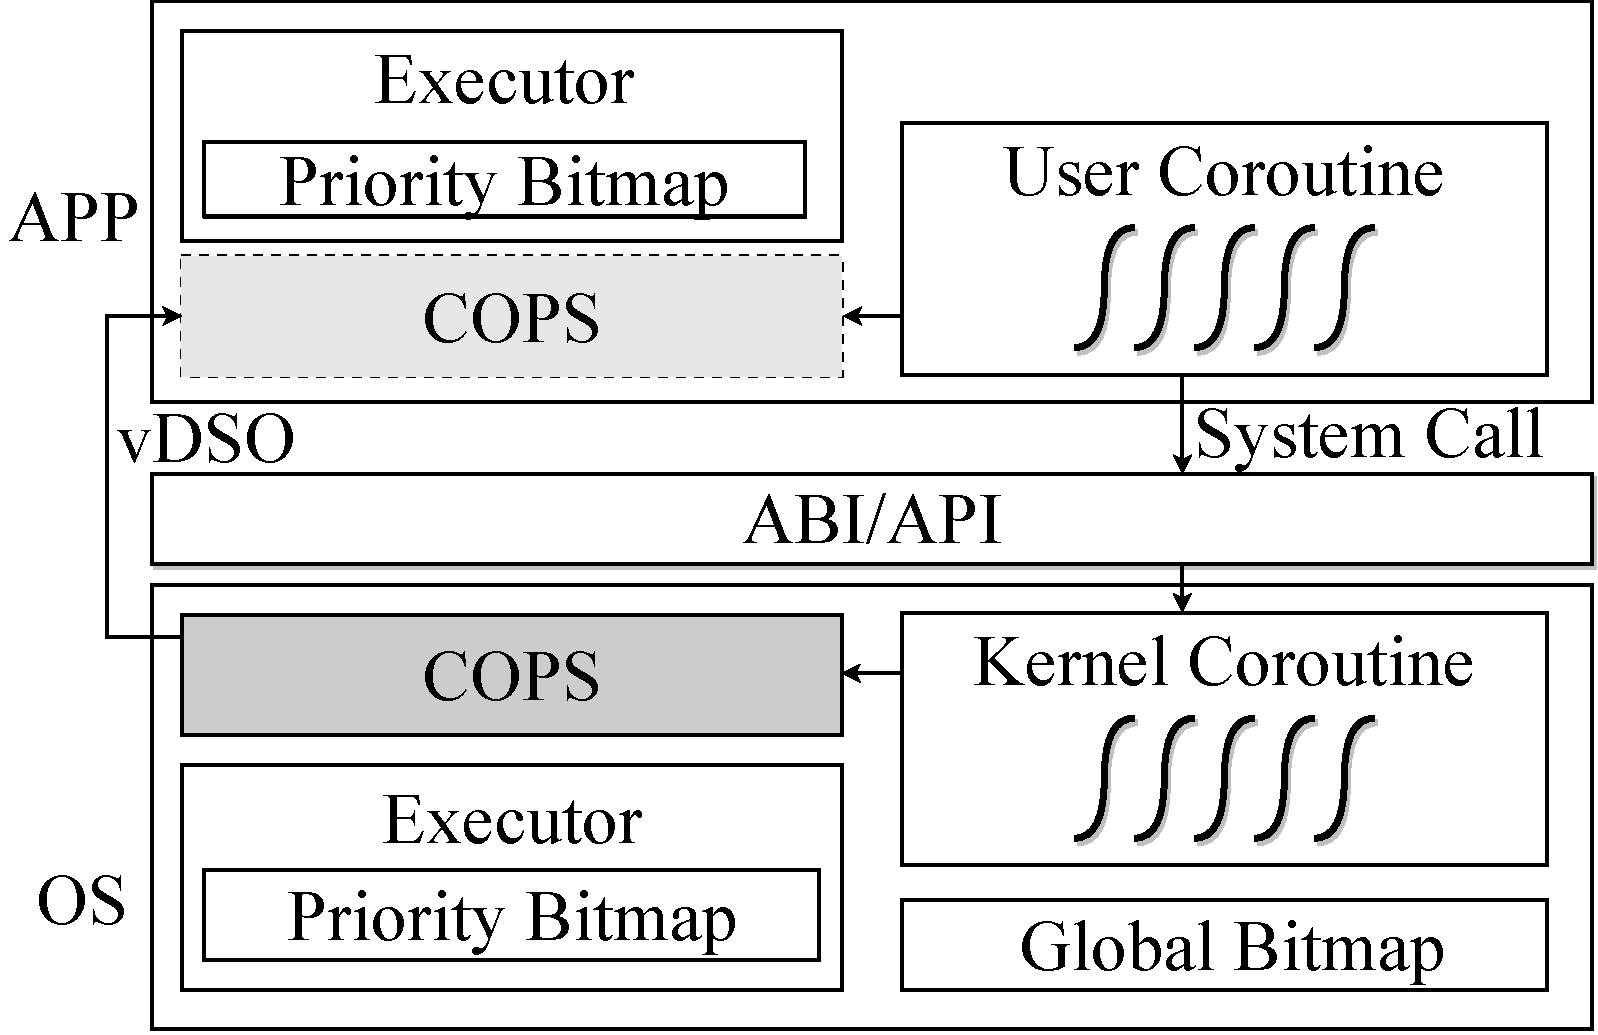
\includegraphics[width=\linewidth]{assets/arch.pdf}
  \caption{The architecture of COPS.}
  \label{fig:arch}
  \Description{The architecture of COPS.}
\end{figure}

Next, we will cover the design details of COPS in the rest of this section. We will first introduce the data structure related to the coroutine runtime provided in COPS to describe how to implement the scheduling of coroutines(\ref{section: Coroutine Runtime}). Next, we will introduce the state transition model of the coroutines(\ref{section: state-transition}). Then, we will describe the COPS API(\ref{section: cops api}). Finally, we will describe the global cooperative scheduling mechanism provided by COPS(\ref{section: global-cooperative-scheduling}).

\subsection{Coroutine Runtime}
\label{section: Coroutine Runtime}

The \textbf{Future} and \textbf{Wake} traits are provided by Rust to support the coroutine mechanism without limiting the specific runtime implementation. Therefore, we can use this decoupling property to customize a coroutine runtime that can be used in both kernel and userland. The Coroutine runtime is mainly composed of the following two parts: 1) Coroutine Control Block; 2) Executor.

\subsubsection{Coroutine Control Block}

As the description of \ref{subsection: rust_async}, the polling process specified in future trait is partially transparent, which prevents us from accurately controlling the coroutine. Therefore, on the basis of future and waker abstractions provided by Rust language, we add additional fields to form coroutine control blocks, so as to achieve precise control of coroutines. The structure of the coroutine control block is shown in listing \ref{ccb}.

How to switch and save the context of the coroutine is the most important issue. The Wake trait is responsible for saving and switching context of coroutine. Both the execution and the context-switching of the coroutine are done by the compiler and are transparent. Therefore, the future and wake must be described in the coroutine control block. However, using these two fields alone means that the execution of coroutine can only use a rough polling way to promote, neither cannot achieve the purpose of accurately control, nor be combined with asynchronous I/O mechanisms to truly take the advantages of coroutines. For this purpose, we use three additional fields in the coroutine control block to achieve the accurately control of the coroutine. 1) The cid is used to identify coroutine control blocks, and plays a key role in asynchronous I/O mechanism; 2) The Kind field is used to indicate the type of the coroutine task. After promoting the execution of the coroutine to a certain stage, COPS will process the coroutine differently according to the task type; 3) The Priority field indicates the priority of coroutine and serves as the basis of the COPS's scheduling framework.

\begin{listing}
\caption{Coroutine control block.}
\label{ccb}
\begin{mdframed}
\begin{minted}[linenos=false,breaklines]{rust}
pub struct Coroutine{
  pub cid: CoroutineId,
  pub kind: CoroutineKind,
  pub priority: usize,
  pub future: Pin<Box<dyn Future<Output=()> + 'static + Send + Sync>>, 
  pub waker: Arc<Waker>,
}
\end{minted}
\end{mdframed}
\end{listing}

Note that we didn't label the coroutine with a state field because the Rust coroutines only have pending or ready states, so the state of the coroutine is implicitly described by the queue it is in.

\subsubsection{Executor}
\label{subsubsection: executor}

The main part of the coroutine runtime is the Executor, which is based on the coroutine control block and is responsible for managing all coroutines within a process. Its main structure includes the following parts:

\begin{itemize}[leftmargin=*]
    \item[1)] Ready queues and priority bitmaps: The Executor maintains ready queues of different priorities, and coroutines are stored in queues corresponding to their priorities. This guarantees that the coroutine with the highest priority can be executed firstly every time. In addition, the Executor maintains a priority bitmap structure corresponding to the ready queue to indicate the presence or absence of coroutines at the corresponding priority level. Although it is unnecessary to maintain this structure in user process Executor, this structure serves the purpose of scheduling within the operating system. Through this data structure, the operating system will gain a certain degree of awareness of user-level coroutines.
    \item[2)] Blocking set: All coroutines that are blocked after execution will be managed by this structure until the event that the coroutine is waiting for occurs and then wakes up from this set.
\end{itemize}

These two data structures provide the runtime environment of coroutines, and provide a basic priority scheduling mechanism for COPS, which ensures that the coroutine priority scheduling in COPS can play a role in the address space of a single process and can be scheduled to the coroutine with the highest priority each time.

\subsection{Coroutine State Transition Model}
\label{section: state-transition}

The introduction of coroutines into the asynchronous I/O mechanism in the kernel to replace the original multithreading model has undoubtedly brought new changes to the basic concepts of process and thread in the operating system. In the case of kernel page table isolation (KPTI) \cite{kpti}, the kernel can also be regarded as a special process, which means that the address space will be switched when entering the kernel and returning to user process. As for thread, its role has been greatly diminished, no longer as the basic unit of task scheduling, only to provide a running stack for coroutines, and as a parallel abstraction of multiprocessor systems. Therefore, the traditional thread state model is no longer needed in task scheduling, instead of the coroutine state model.

Similar to the thread state model, coroutines have five basic states: create, ready, running, blocked, and exit, but there is also a special state: the running-suspended state. This is due to the preemptive scheduling provided by the operating system and some other special cases. The coroutine only has the stack when it is in the running state, but the execution process of the coroutine in the running state may be interrupted by clock interruption, exception, or entering the kernel to perform synchronous system calls. In this case, the coroutine will occupy the running stack in a certain time scale, but it is no longer in the state of executing on the CPU, so we define it as the state of running-suspended. According to the cause, it can be further divided into operation interrupt state and operation exception state. The coroutine state transition model is shown in Fig.~\ref{fig:state}.

\begin{figure}[h]
  \centering
  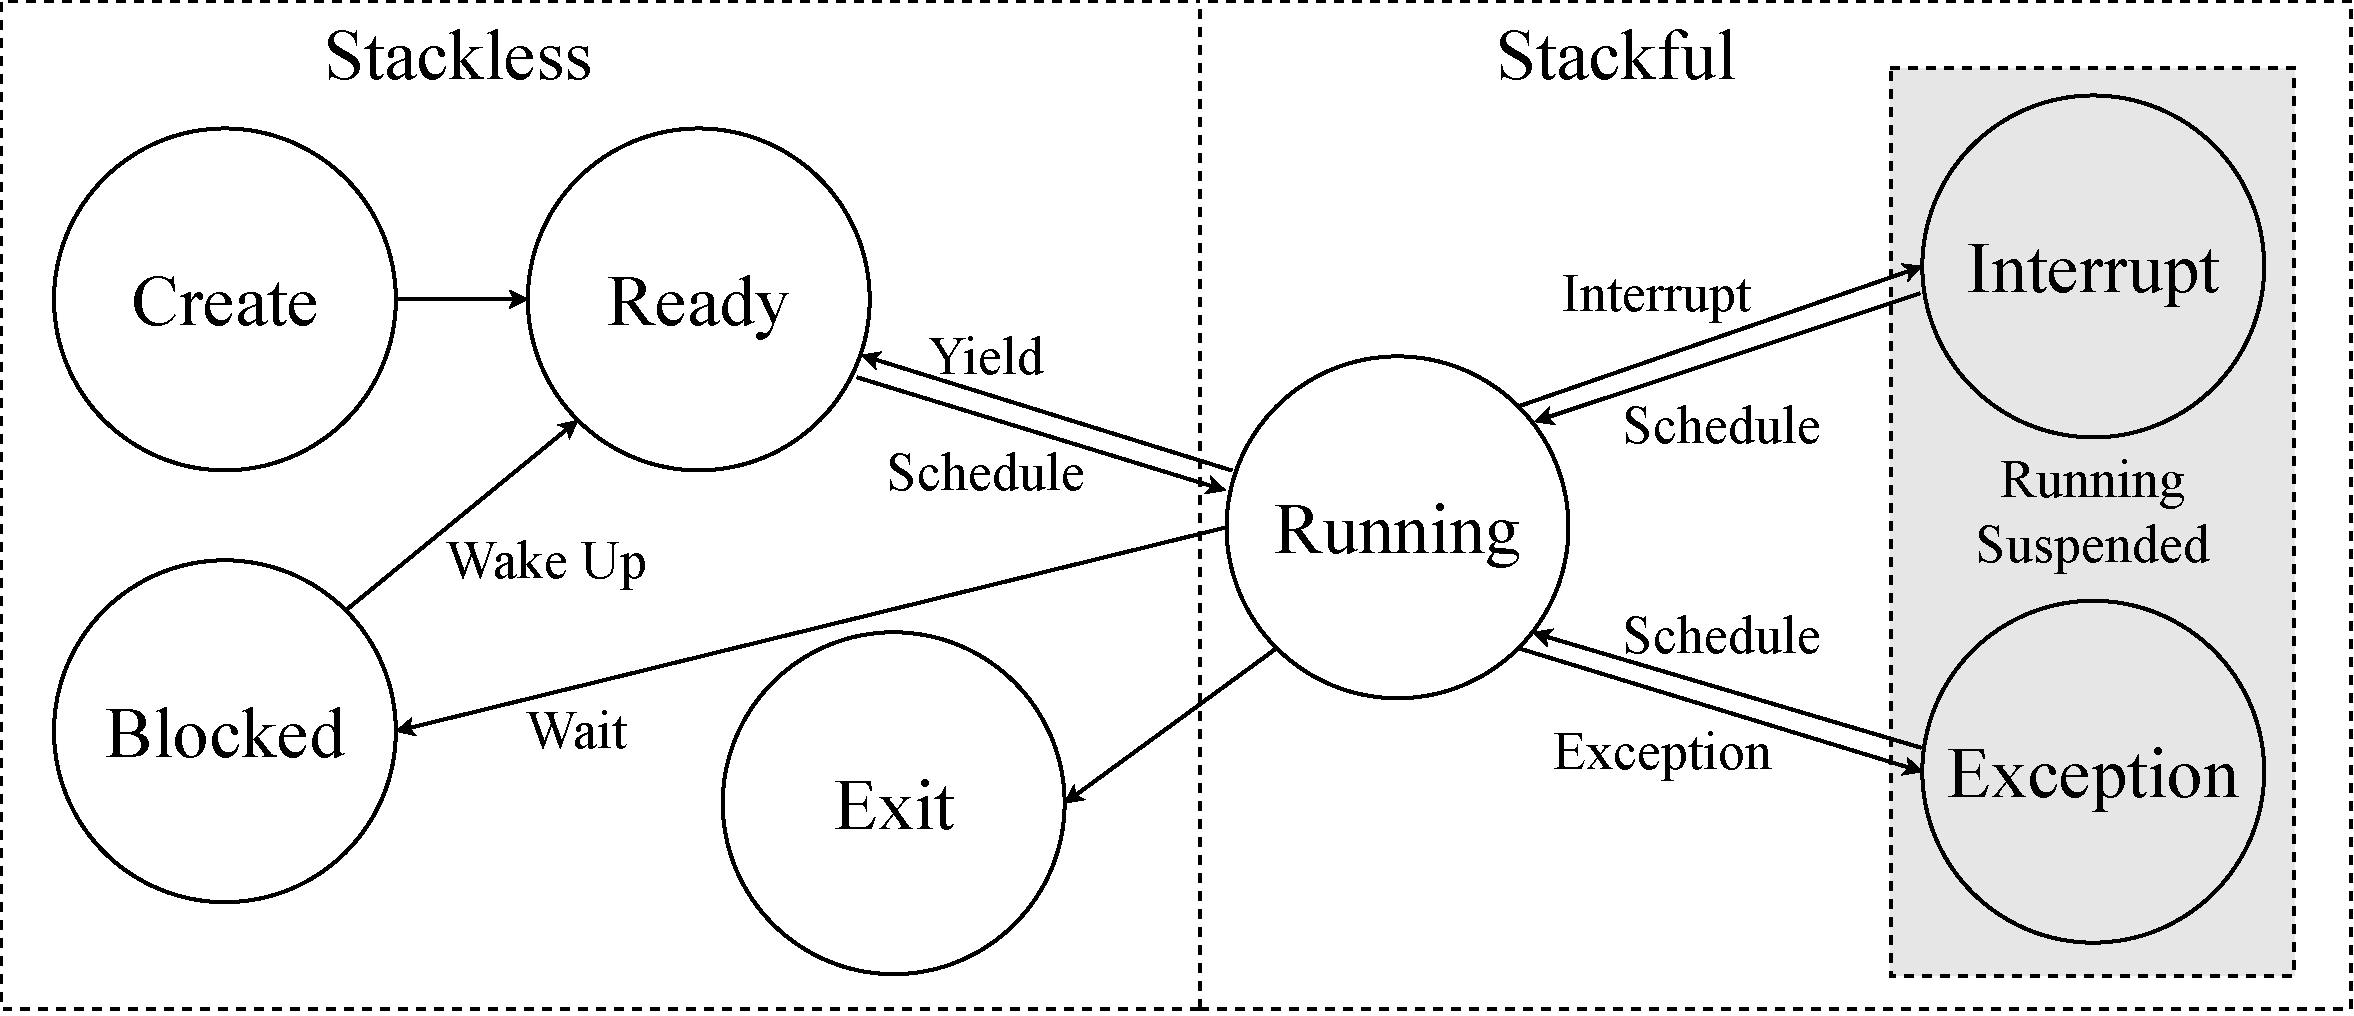
\includegraphics[width=\linewidth]{assets/cstate.pdf}
  \caption{Coroutine state transition model.}
  \label{fig:state}
  \Description{Coroutine state transition model.}
\end{figure}

\begin{enumerate}[leftmargin=*]
    \item Once a coroutine is created, it goes into the ready state until it is scheduled and thus into the running state.
    \item For a coroutine in the running state, the possible state transitions can be divided into two categories. On the one hand, it may wait for an event to enter the blocked state, or it may yield actively and turn to ready state when detecting other coroutines with higher priority (including coroutines in other processes). This type of state transition does not occupy the running stack; On the other hand, if an interrupt or exception occurs during the running, the CPU will be preempted and the current coroutine will enter a running-suspended state. In addition, when the task is completed, the running coroutine will enter the exit state, waiting for the resource to be reclaimed.
    \item When the coroutine is in the blocked state, it must wait for an event to wake itself up and thus enter the ready state. However, when the coroutine is in the running-suspended state, it does not need to go through the ready state transition, and only needs to wait for the relevant handling to complete before entering the running state.
\end{enumerate}

\subsection{COPS API}
\label{section: cops api}

According to the general definition of coroutines, the coroutines has three basic operators: \textit{create}, \textit{resume} and \textit{yield}. In Rust, the \textit{resume} and \textit{yield} operators are replaced by the poll function and the await keyword, respectively. Since the future must be driven by await keyword, it is not necessary to consider whether the \textit{yield} is placed in the right places. Certainly, we cannot avoid that the developer may accidentally use a tight loop in the coroutine, which will cause the coroutine to occupy the CPU for a long time. Pure cooperative scheduling frameworks are helpless against this dilemma. However, COPS can deal this dilemma through a global cooperative scheduling mechanism. This will be introduced in the section \ref{section: global-cooperative-scheduling}.

COPS provides the \textit{spawn} operator to create a new coroutine. Besides, COPS also provides additional interfaces(\textit{current, wake\_up, set\_priority, alloc\_cpu}) to enhance the control capability of coroutines. The \textit{spawn} function create a new coroutine in the current process(kernel) and return the identity of the new coroutien. The first argument is the closure of the coroutine main body. The \textit{current} function returns the identity of the current coroutine. The \textit{wake\_up} function wakes up the coroutine with the specified identity. And the \textit{set\_priority} function sets the priority of the coroutine with the specified identity. The \textit{alloc\_cpu} function is used to apply for more CPU resource. Default, an application is only allocated one CPU. Developers can call the \textit{alloc\_cpu(1)} to apply for an additional CPU for the current application. Table \ref{tab:interface} shows the interfaces provided by COPS.

Using the COPS API, developers can take advantage of coroutine at mostly without any restrictions, no matter in the kernel or user space.

\begin{table}[]
  \begin{tabular}{@{}cc@{}}
  \toprule
  Function                     & Return Value \\ \midrule
  spawn(future, priority)      & cid          \\
  current()                    & cid          \\
  wake\_up(cid)                &              \\
  set\_priority(cid, priority) &              \\
  alloc\_cpu(cpu\_num)          &              \\ \bottomrule
  \end{tabular}
  \caption{Interface of COPS.}
  \label{tab:interface}
  \vspace{-3em}
\end{table}

\subsection{Global Cooperative Scheduling Mechanism}
\label{section: global-cooperative-scheduling}

On the basis of the coroutine priority scheduling, COPS also provides a more advanced global cooperative scheduling mechanism: cooperative scheduling between the kernel and user processes and cooperative scheduling between user processes. The priority bitmap mentioned in \ref{subsubsection: executor} plays a key role in this process.

The first is the coordination between the coroutines in the kernel and the coroutines in the user process. When the kernel handles the time interrupts, it scans the priority bitmap in all user process Executor to generate a global priority bitmap, so that the operating system can perceive the user-level coroutine to a certain extent. There is also an Executor in the kernel to manage the kernel coroutines. Coordination between the operating system and user processes can be achieved by combining the global priority bitmap with the priority bitmap in the kernel Executor. In the process of coordination, kernel task scheduling is divided into coroutine scheduling and process scheduling. The most directly way to achieve this goal is to define a process scheduling and a coroutine scheduling separately, which can ensure that coroutines with high priority in the kernel are executed first, and then to determine the execution of user processes. However, this extra mechanism can bloat the system and does not solve the problems with the kernel asynchronous I/O mechanism mentioned in \ref{section: introduction}. A more elegant design that can solve this problems is to introduce a special coroutine in the kernel: the switching coroutine. The switching coroutine is responsible for finding the user process with the highest priority and completing the switching operation, so it never ends as long as there is a user process. Its priority is consistent with the highest priority of all processes, so as to ensure that the scheduling of kernel coroutines and user processes can be cooperative according to the priority. When the kernel is initialized, it is staticly assigned the highest priority, then its priority changes dynamically once the system is running. The kernel determines the priority of the switching coroutine after scanning the priority bitmap. In this case, process and coroutine scheduling in the kernel can reuse the priority scheduling mechanism provided by COPS. When there are other coroutines with higher priority in the kernel, it means that all the coroutines within the user process are inferior to the coroutines in the kernel, need to wait for the kernel to finish executing the coroutine with higher priority. Then the process with the highest priority can be scheduled by switching coroutine. This ensures coordination between kernel coroutines and user processes.

In addition, we share the read-only permission of the above global priority bitmap with the user process, so as to achieve the coordination between coroutines in different processes. Once the user process detects the existence of a higher priority coroutine in the operating system or other processes while it is running, the user process will yield actively to achieve mutual coordination. However, blind global coordination may cause some malicious processes to occupy CPU for a long time or cause frequent switching overhead, which will be our future improvement direction, and this problem is not covered in this paper.

Through the above mechanism, COPS provides an operating system aware coroutine-based scheduling framework, which can avoid one coroutine occupying CPU for a long time. Fig.~\ref{fig:flow} shows the code logic of COPS.

\begin{figure}[h]
  \centering
  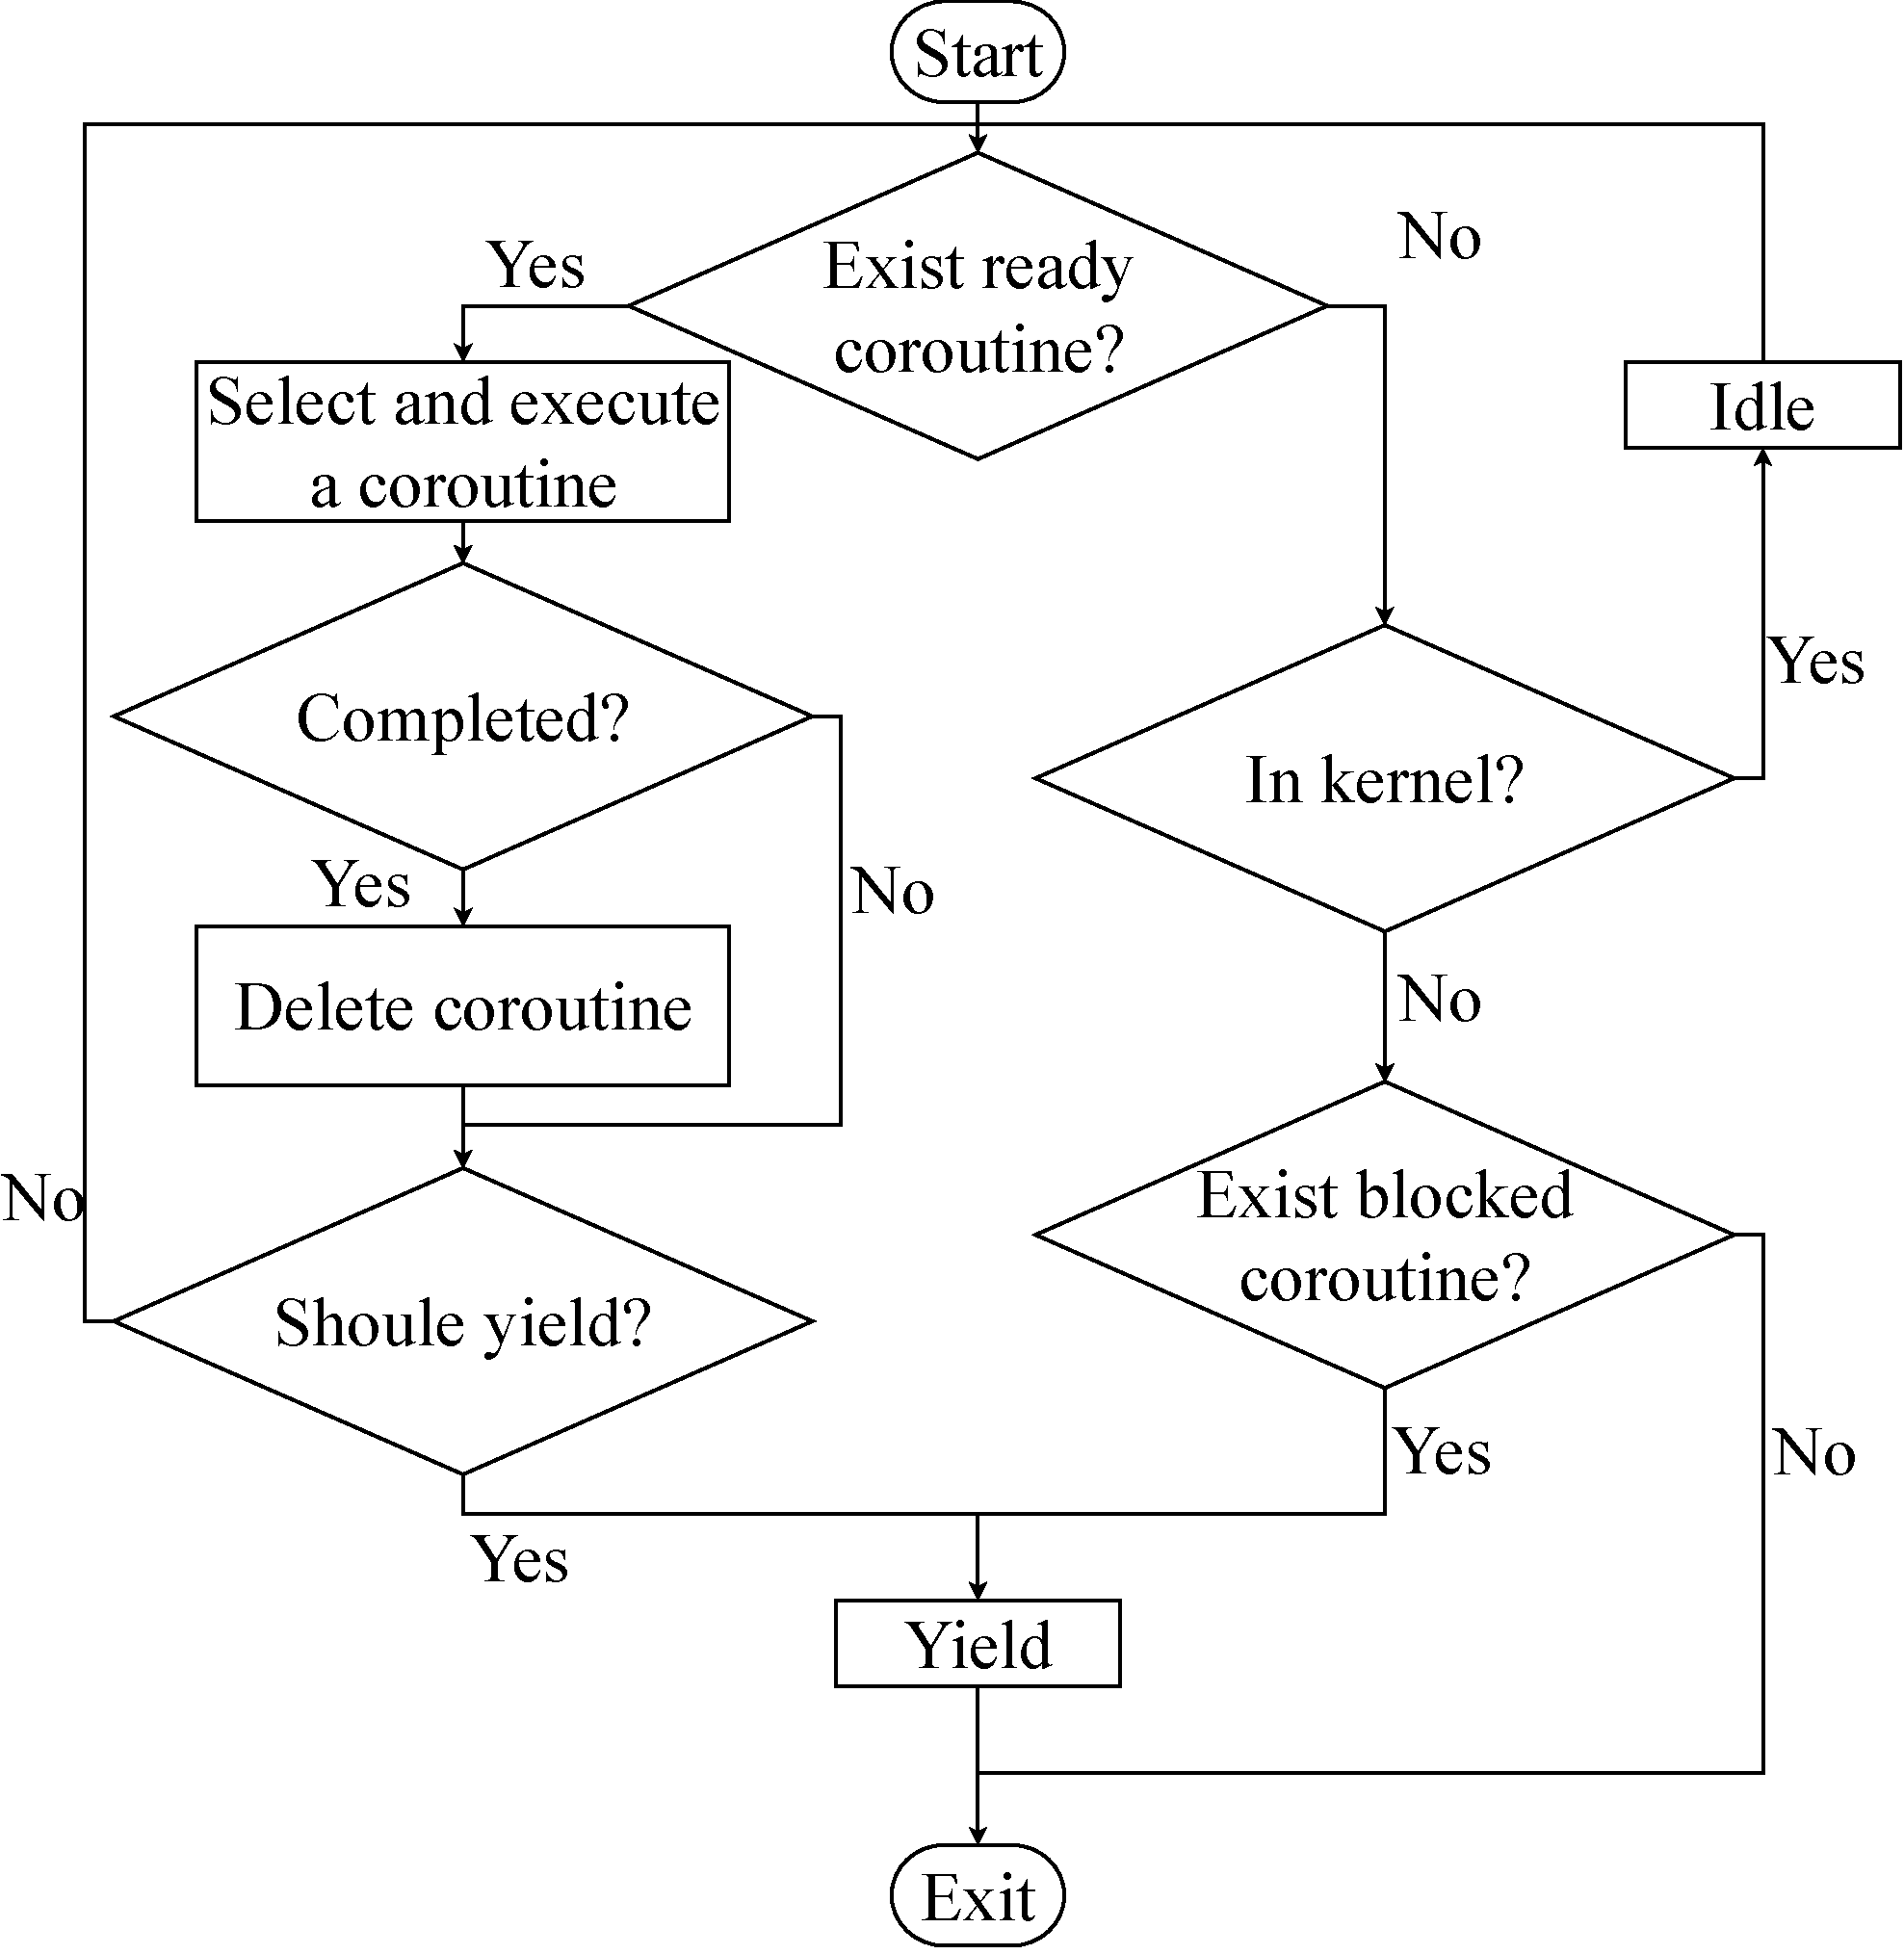
\includegraphics[width=\linewidth]{assets/flow.pdf}
  \caption{The code logic of COPS.}
  \label{fig:flow}
  \Description{The code logic of COPS.}
\end{figure}

\section{Common usage patterns}
\label{section: Common usage patterns}

In this section, we illustrate COPS use patterns for concurrent and asynchronous programming. Both the patterns are broadly applicable. COPS provides an environment that all tasks exist in the form of coroutines. What the main body of application needs to do is using the \textit{spawn} function to create coroutines with specific functionality. The running of coroutines is transparently driven by the coroutine runtime provided by COPS.

\subsection{Concurrency}

A common COPS use pattern is to build a producer-consumer model, shown in Algorithm \ref{alg: concurrency}, where the application creates two coroutines: one producer and one consumer. The producer will firstly be driven by COPS to produce data. While the message queue is full, the producer will wake up the consumer and yield the CPU. Then, consumer will consume all data and block itself. Next, COPS will schedule the producer again.

\begin{algorithm}[!h]
  \caption{Concurrent Programming}
  \label{alg: concurrency}
  \begin{algorithmic}[1]
    \State $MSG\_QUEUE;$
    \Function{main}{}
      \State $consumer\_cid \gets spawn(|| consumer, 1)$;
      \State $spawn(|| producer(consumer\_cid), 0)$;
		\EndFunction

    \Function{consumer}{}
      \Loop
        \While{MSG\_QUEUE is empty}
          \State blocked;
        \EndWhile
        \State ... \Comment{consume data from MSG\_QUEUE}
      \EndLoop
    \EndFunction

    \Function{producer}{cid}
      \Loop
        \While{MSG\_QUEUE is full}
          \State wake\_up(cid); \Comment{wake up the consumer}
          \State yield;
        \EndWhile
        \State ... \Comment{produce data into MSG\_QUEUE}
      \EndLoop
    \EndFunction
  \end{algorithmic}
\end{algorithm}

\subsection{Asynchronous Programming}

Another common COPS usage pattern is for asynchronous programming. COPS provides a coroutine runtime environment, so asynchronous programming can be achieved by simply transforming the original synchronous system call into an asynchronous system call based on coroutines. However, it is not enough to modify the interface form alone, and support for asynchronous system calls must also be implemented in the kernel.

\begin{itemize}[leftmargin=*]
  \item[1)] System call interfaces: In order to ensure that system calls can support asynchronous features, we add an \textbf{Asyncall} auxiliary data structure that implements the future trait specified in Rust, and this data structure will determine whether asynchronous waits are required according to the value returned by the system call. In addition, we use the macro mechanism in Rust to ensure that synchronous and asynchronous system calls are similar in form. The difference between the two is that an asynchronous system call requires an additional parameter. We show the read system call interface in listing \ref{listing: system call}.
  \item[2)] Kernel asynchronous I/O support: When a user-level coroutine invokes an asynchronous system call, the kernel will create a kernel coroutine corresponding to the user-level coroutine, which it is not be executed immediately. Then the control flow will immediately return to the user-level coroutine, blocking the current coroutine so that other user-level ready coroutines can continue to execute. Once the kernel has executed the coroutine and completed the corresponding asynchronous operation, it will wake up the corresponding user-level coroutine with the cid passed by the system call. 
\end{itemize}

Algorithm \ref{alg: asynchronous programming} shows how to use the asynchronous system call interface for asynchronous programming. In the async\_read function, it calls the \textit{read!} system call interface for asynchronous reading. If there is no data in the kernel buffer, the async\_read coroutine will give up the CPU. Once there is data in the kernel buffer, the async\_read coroutine will be waked up.

\begin{algorithm}[!h]
  \caption{Asynchronous Programming}
  \label{alg: asynchronous programming}
  \begin{algorithmic}[1]
    \Function{main}{}
      \State $spawn(|| async\_read, 0)$;
		\EndFunction

    \Function{async\_read}{}
      \State $buf \gets [0; buf\_len]$;
      \State $current\_cid \gets current()$;
      \State $read!(buf.ptr, buf.len, current\_cid)$;
    \EndFunction
  \end{algorithmic}
\end{algorithm}

\begin{listing}
  \caption{System call interface of read().}
  \label{listing: system call}
  \begin{mdframed}
  \begin{minted}[linenos=false,breaklines]{rust}
  read!(fd, buffer, cid); // Async call
  read!(fd, buffer); // Sync call
  \end{minted}
  \end{mdframed}
\end{listing}

\begin{figure}[h]
  \centering
  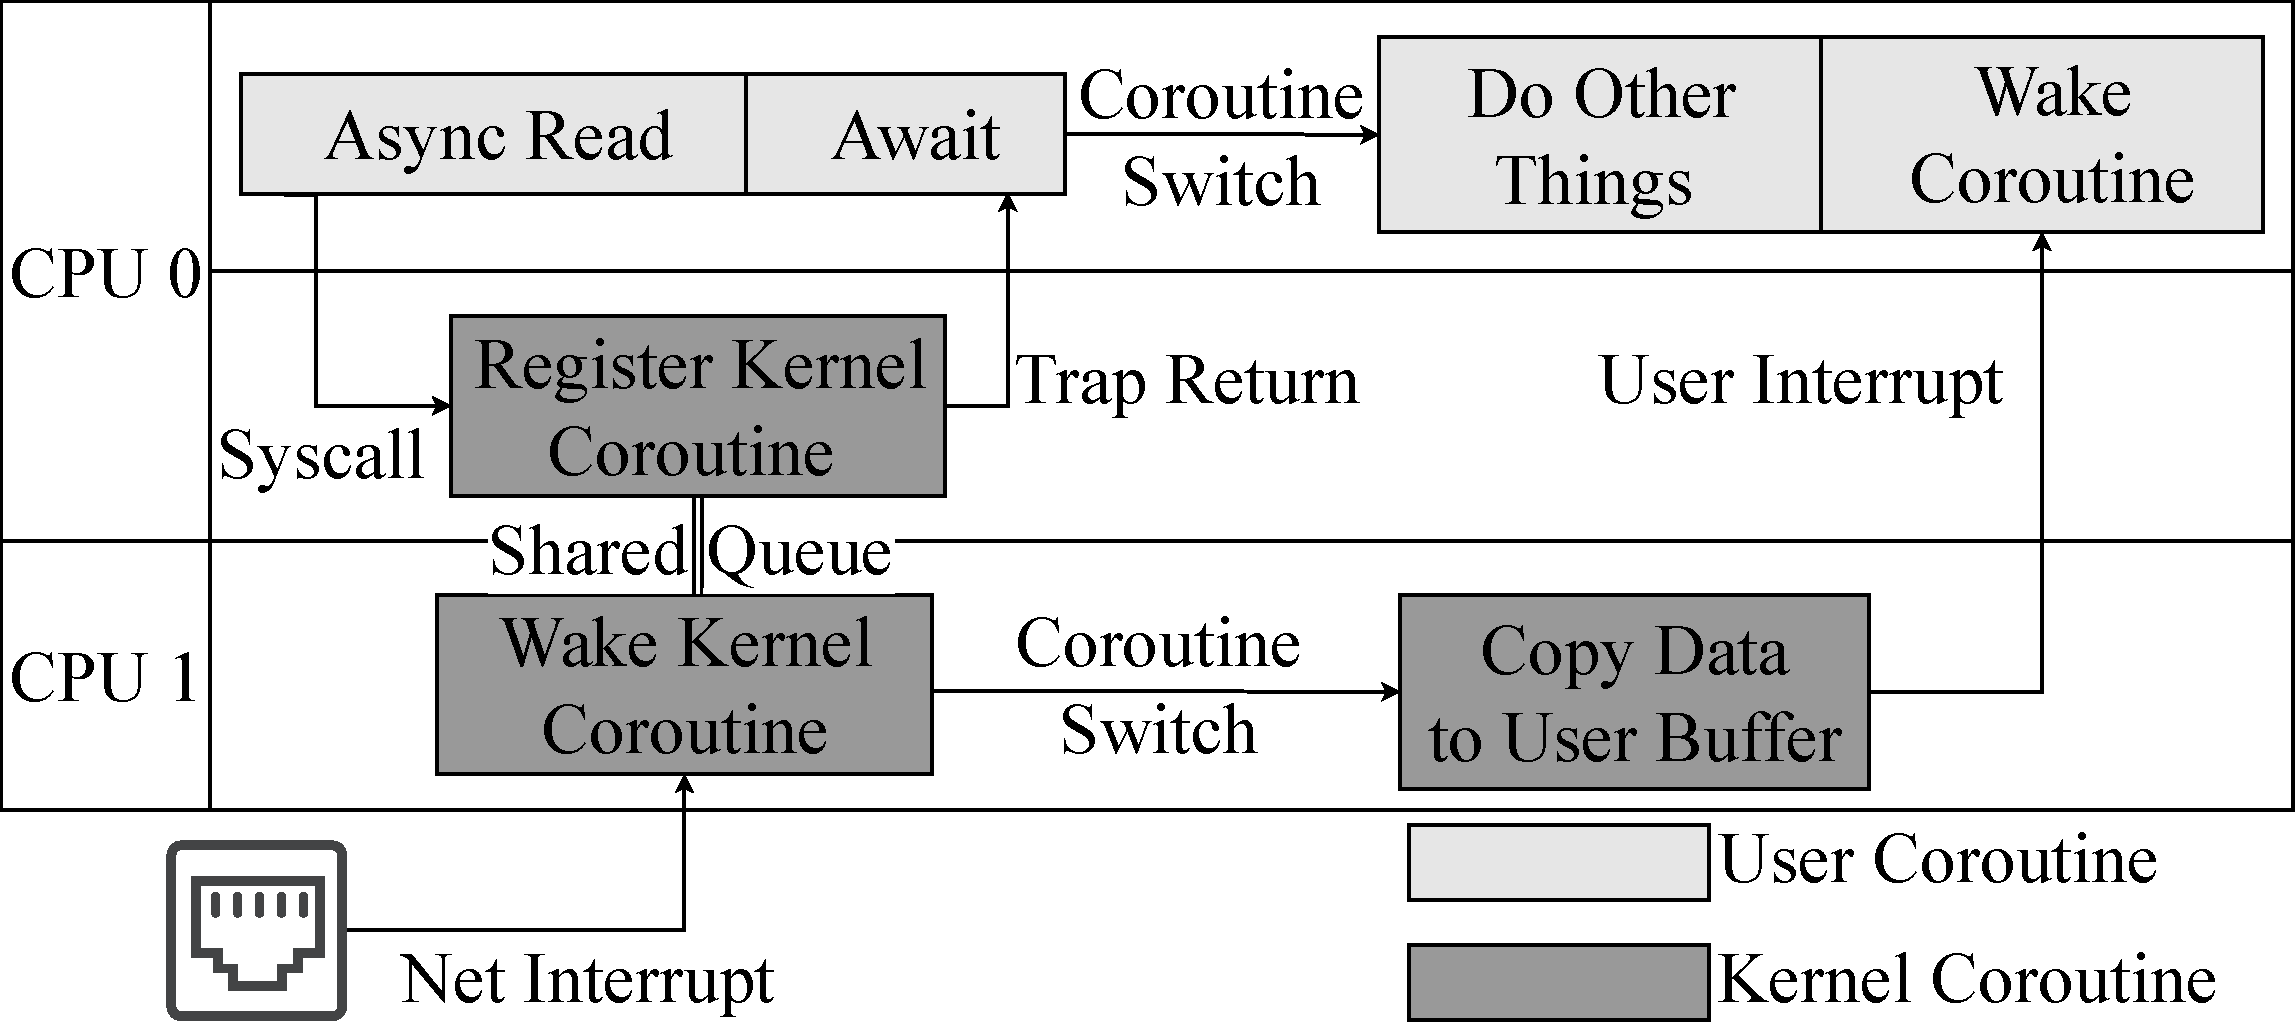
\includegraphics[width=\linewidth]{assets/async_syscall.pdf}
  \caption{Asynchronous system call.}
  \label{fig:async_syscall}
  \Description{Asynchronous system call.}
\end{figure}

In order to illustrate that how coroutines can be combined with asynchronous I/O mechanism, we use the example of asynchron-ously reading data from sockets. Once inside the kernel, the operations that were previously done synchronously by the kernel are encapsulated in the kernel coroutine. The control flow then immediately returns to user space and blocks the current coroutine, waiting for the kernel to finish reading operation. At this point, COPS switches and executes the next user coroutine. The kernel coroutine can be executed on another CPU. As if the data in this buffer is already ready, the kernel coroutine does not need to wait, which takes full advantage of the multi-processor; If the data in the buffer is not ready, the kernel coroutine will be blocked and wait for the network card to wake itself up. while the other kernel coroutines will be able to continue executing. Once the kernel has received the interrupt generated by the network card and has prepared the data in the buffer, the corresponding kernel coroutine is woken up to continue execution. Once the kernel coroutine finishes its work (in this case, copying data to the user-space buffer), it sends a user-level interruption, telling the user-level interruption handler to wake up the corresponding coroutine.

\section{Performance Evaluation}
\label{section: Performance Evaluation}

In order to verify the effectiveness of COPS in building highly concurrent asynchronous programs and more accurate control of coroutines, we set an evaluation in FPGA. The FPGA model is Zynq UltraScale+ XCZU15EG-2FFVB1156 MPSoC \cite{zynq}. We build a five-level RISC-V pipelining processor, which is based on the rocket-chip \cite{rocket-chip} (a RISC-V soft IP core), in FPGA. Since asynchronous system calls relys on the relevant functions of user-level interruption, we implement N extension \cite{waterman_volume_nodate} on rocket-chip. We run an operating system based on COPS framework on the RISC-V subsystem, and finally complete the evaluation of COPS by simulating the real web server application scenario. The total configuration parameters are shown in Table \ref{tab:cfg}.

\begin{table}
  \begin{tabular}{|c|c|c|}
    \hline
    \multirow{3}{*}[-0.5cm]{FPGA} & \multicolumn{2}{c|}{ \makecell{Zynq UltraScale+ \\ XCZU15EG-2FFVB1156 MPSoC \cite{zynq}}} \\                             \cline{2-3}
                          & \makecell{RISC-V \\ soft IP core} & \makecell{ rocket-chip \cite{rocket-chip} with N \\ extension, 4 Core, 100MHz } \\ \cline{2-3}
                          & \makecell{Ethernet \\ IP core} & \makecell{Xilinx AXI 1G/2.5G \\ Ethernet Subsystem (1Gbps) \cite{axi-eth} } \\ \cline{2-3}
    \hline
    \makecell{Operating \\ System} & \multicolumn{2}{c|}{ rCore-tutorial\cite{rcore-os/rCore-Tutorial-v3} } \\ \cline{2-3}
                            
    \hline
    \makecell{Network \\ Stack} & \multicolumn{2}{c|}{ smoltcp\cite{smoltcp} } \\
    \hline
  \end{tabular}
  \caption{Configuration of evaluation.}
  \label{tab:cfg}
  \vspace{-3em}
\end{table}

The simulated web server application scenario consists of two parts. One part is the client running on PC, sending a certain length of matrix data to the server regularly, and receiving the response from the server. The other part is the server in the FPGA, combined the two usage patterns, which establishes a connection with the client, performs matrix operations on the matrix data sent by the client and returns the results to the client. The server has the following three components:

\begin{enumerate}[leftmargin=*]
    \item Receiving request component: It receives the request from the client and stores it in the request queue;
    \item Handling Request component: It removes the request from the request queue, performs matrix operations, and stores the result in the response queue;
    \item Sending response component: It retrieves the response message from the response queue and sends it to the client.
    
\end{enumerate}

Finally, the client on the PC calculates the time latency between sending each request and receiving the response, and calculates the throughput of messages within a fixed period of time. We evaluate COPS by analyzing the time latency and throughput of the web server under different configurations.

\subsection{Coroutine vs. Thread}

To confirm that the coroutine model is more suitable for large-scale concurrency scenario, we use coroutines and threads in the kernel and application respectively to implement the three components of the web server mentioned above. Using the coroutine model creates three coroutines for each connection between the client and the server, while using the thread model creates three user threads for each connection, corresponding to the three components mentioned above. The web server can be divided into four models based on the combination of coroutines and threads used in the kernel and applications. \textbf{K} means in the kernel and \textbf{U} means in the userland. \textbf{C} means using coroutines and \textbf{T} means using threads. Note: The threads used in the application are kernel-supported threads. 

\textbf{KCUC}: When the user-level coroutine invokes read() system call, the kernel will create a kernel coroutine to execute the operations and the current user-level coroutine will be blocked. Once the kernel coroutine reads data from the socket and completes the copy operation, the kernel coroutine will send a user-level interruption to wake up the corresponding user-level coroutine.
	
\textbf{KCUT}: When the user thread in userland invokes read() system call, it is similar to KCUC, the kernel will create a kernel coroutine to execute the operations and block the current user thread. The kernel coroutine will wake up the blocked thread after the copy operation is completed.
	
\textbf{KTUT}: The user thread invokes the read() system call, and the corresponding kernel thread will continue to try to read data from the socket until the data copy operation is completed before returning to the user space to continue executing, during which other threads can be executed.
	
\textbf{KTUC}: Similar to kcuc, but it no longer completes the copy operation through the kernel coroutine, instead of submitting the information of the reading operation to another separate kernel thread and directly returns to the userland. This kernel thread will constantly poll all the socket ports submitted by the user coroutines and copy data from the socket which has data in the buffer. After the data replication operation is completed, it will send a user-level interruption to wake up the corresponding user coroutine.


The test start after all connections between the client and the server are established, to eliminate the impact of coroutine/thread creation. The client sends requests to the server every 100ms for 5s, and the matrix size of each request is 15 x 15. The experimental results are as shown in Fig.\ref{fig:throughput-latency}.

\begin{figure}[ht]
  \Description[]{Throughput and message latency.}
	\centering
	\subcaptionbox{Throughput\label{subfig:throughput}}[0.49\linewidth]
	{
		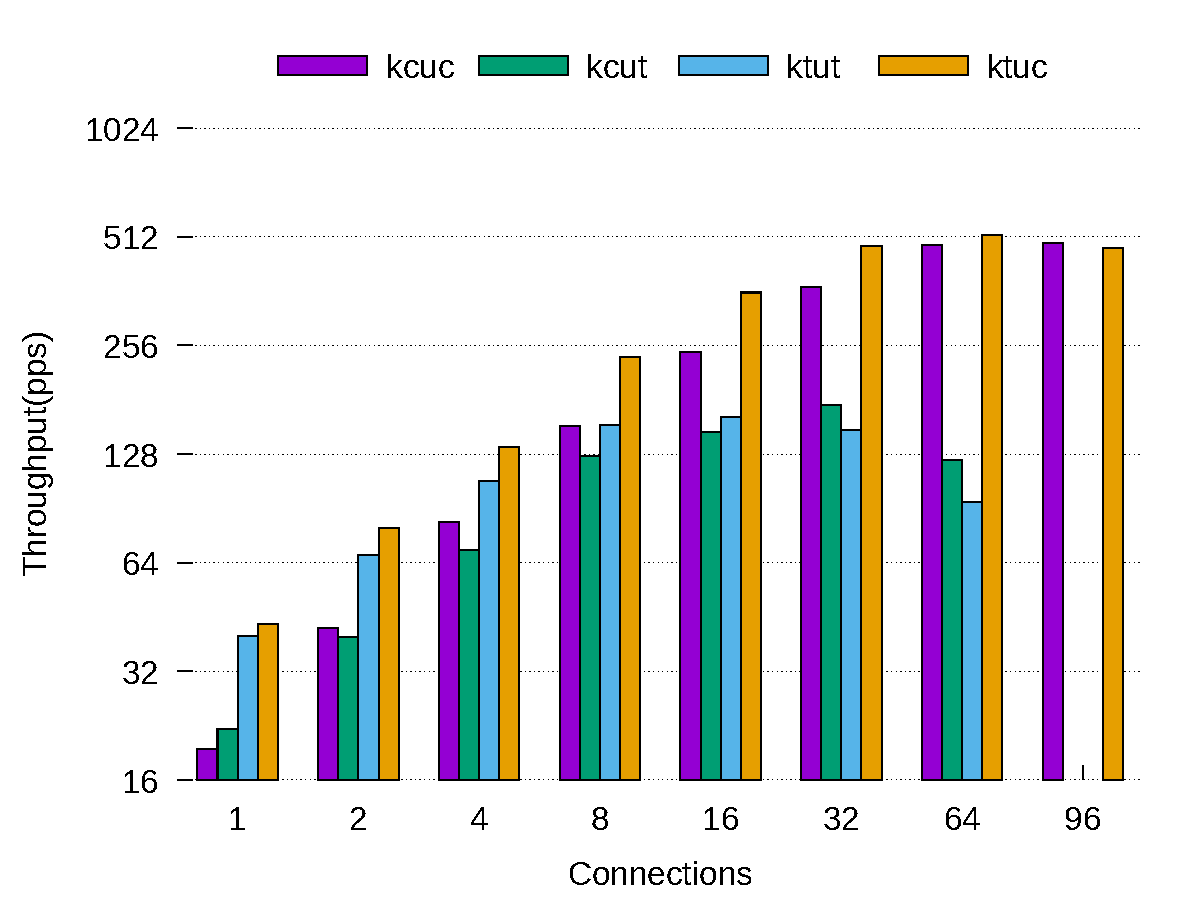
\includegraphics[width=\linewidth]{assets/throughput.pdf}
	}
	\subcaptionbox{Latency\label{subfig:latency}}[0.49\linewidth]
	{
		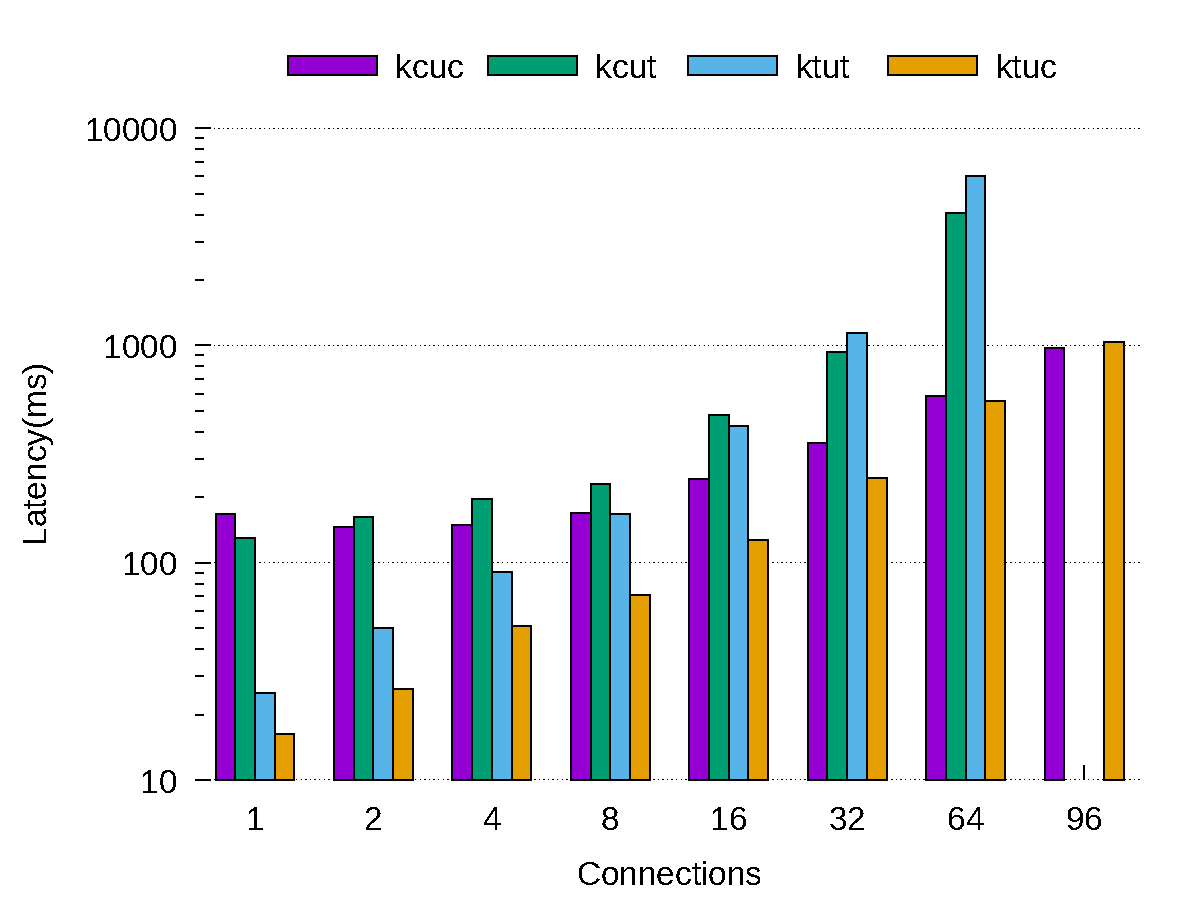
\includegraphics[width=\linewidth]{assets/latency.pdf}
	}
	\caption{Throughput and message latency.}
	\label{fig:throughput-latency}
\end{figure}

\textbf{Runtime overhead}: When the amount of connections is small, using coroutines will cause more overhead than using threads. This can be seen from the comparison of KCUC vs KCUT, KCUT vs KTUT, and KCUC vs KTUT in Figure \ref{fig:throughput-latency}. This is because the executor of COPS's runtime is protected by a lock. When the amount of connections is small, COPS requires only a small number of cores to complete the task, but it is allocated extra CPU for a fair comparison(The number of cores allocated to coroutine model is the same as the thread model). On the one hand, the allocation of excess CPU will cause extra synchronous mutual exclusion overhead when scheduling the coroutines; On the other hand, COPS on the extra core will yield frequently because of no ready coroutine which will cause the overhead of privilege level switching. Therefore, COPS is not applicable to applications with low concurrency.

\textbf{Lower coroutine context-switching overhead}: According to KCUC vs KCUT and KCUT vs KTUT, the latency of the threading model will gradually exceed that of the coroutine model as the number of connections increases. When the number of connections reaches 32, the latency of KCUT is lower than that of KTUT. The coroutines and threads in the kernel complete the same operation, so the overhead of coroutine context-switching is less than that of threads (even the kernel thread with simplified context switching). When the number of connections is 2, the latency of KCUC is lower than that of KCUT. This is because most of the coroutine context-switching in KCUC model are carried out in userland, while the privilege-switching exist in KCUT model. However, KCUT and KTUT models that use threads will decrease their throughput and increase their context-switching cost rapidly as the number of connections increases to a certain extent.

\textbf{Coroutines have obvious advantages with high concurrency}: when the number of connections is small, the KTUC model has the lowest latency, which is reasonable, KTUC uses a separate kernel thread to constantly poll the state of sockets, and can respond in a timely manner, so the latency is lowest. However, as the number of connections gradually increases, the advantage is no longer obvious, and the overhead of each poll of the KTUC kernel thread gradually increases. From the comparison of throughput, when the number of connections reaches 64, the CPU is running with the full workload. When the number of connections reaches 96, the latency of KCUC model is lower than that of KTUC model (KCUT and KTUT model cannot complete the test due to heavy workload. Figure \ref{fig:throughput-latency} does not show the corresponding throughput and message latency). When the number of connections continues to increase, the throughput of KTUC model decreases significantly, while the throughput of KCUC model does not decrease significantly. Although we did not use a separate thread to complete the data replication operation in our experiment, the analysis shows that the effect of KTUC model will not be significantly improved even if epoll is adopted. On the one hand, epoll requires additional synchronous mutually exclusive overhead because of using producer-consumer model. On the other hand, the overhead of thread context-switching will increase. Therefore, after comparing KCUC with KTUC, we can conclude that COPS is suitable for large-scale concurrent scenario.

\textbf{Less memory usage}: In addition to the comparison of throughput and latency, we also compare the memory usage of coroutines and threads. The user-level threads are kernel-supported, which have two stacks at the same time, one for execution in userland and the other for execution in kernel. Meanwhile, no matter the kernel coroutines or the userland coroutines, they must run on a stack. The stack size is staticly configured as 0x4000 bytes. The size of three components implemented by using coroutines are 120(Receiving request component), 80(Handling Request component) and 64(Sending response component) bytes. The size of kernel coroutine is 176 bytes. Therefore, establishing a connection in the KTUT model needs to occupy 0x4000 * 2 * 3 bytes, while the KCUC model only needs to occupy 0x4000 * 2 + 176 + 120 + 80 + 64 bytes. Table \ref{tab:mem_usage} shows the maximum connections that can be established for the KTUT model and the KCUC model under certain settings.

\begin{table}
  \begin{tabular}{cccc}
    \hline
    Configuration & Size(bytes) & KCUC & KTUT \\ \hline
    kernel heap   & 0x80\_0000  & \multirow{3}{*}{385} & \multirow{3}{*}{186} \\ 
    kernel frame  & 0x1A0\_0000  \\ 
    user heap     & 0x20\_0000   \\ 
    \hline
  \end{tabular}
  \caption{Maximum connections of KCUC and KTUT.\textnormal{The stack used by the thread is allocated from the kernel frame.}}
  \label{tab:mem_usage}
  \vspace{-3em}
\end{table}

\subsection{Priority orientation}

In a real scenario, the web server needs to host tens thousands of connections, but a large part of the connections may be idle. The resources in the system should be biased to those active connections, and higher priority should be assigned to ensuring that these connections can receive timely responses. Therefore, we set the priority level of each connection in a hierarchical manner to ensure that connections with higher priority have lower latency and less latency jitter. Similar to the above experiment, but both the kernel and the application use coroutines. Priority scheduling is implemented by COPS. We set up 64 connections between the client and the server, divided into 8 priorities on average, and test the throughput and message latency of different priority connections in the same time period. The client sends a request to the server every 50ms for 5s. As shown in the Figure \ref{fig:prio-throughput-latency}, the throughput and latency of connections with higher priority levels can be guaranteed under limited resource constraints. As the number of resources increases, the low priority connection can also achieve higher throughput and lower latency, while the connection with the highest priority still has the highest throughput and lowest latency.

\begin{figure}[ht]
  \Description[]{Throughput and message latency of different priority connections.}
	\centering
	\subcaptionbox{Throughput\label{subfig:prio-throughput}}[0.49\linewidth]
	{
		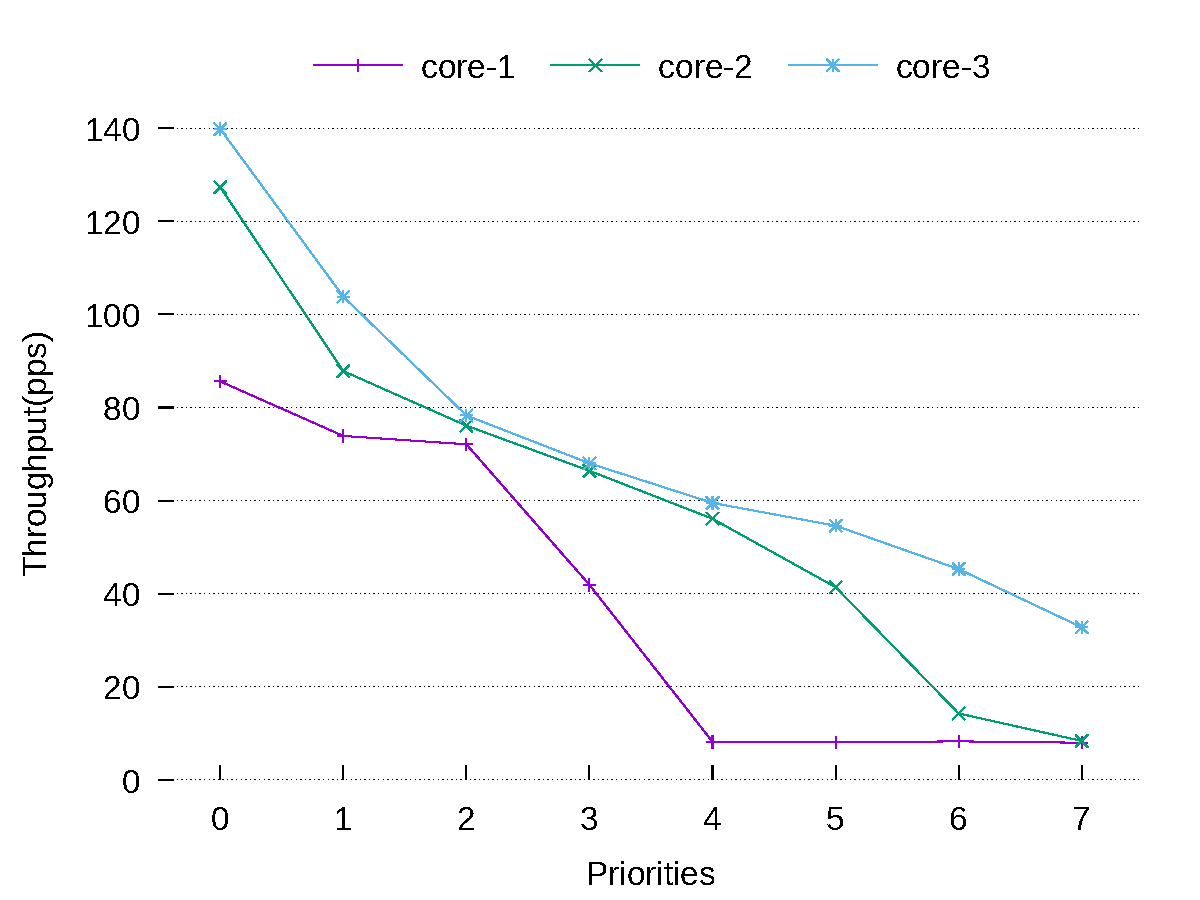
\includegraphics[width=\linewidth]{assets/prio-throughput.pdf}
	}
	\subcaptionbox{Latency\label{subfig:prio-latency}}[0.49\linewidth]
	{
		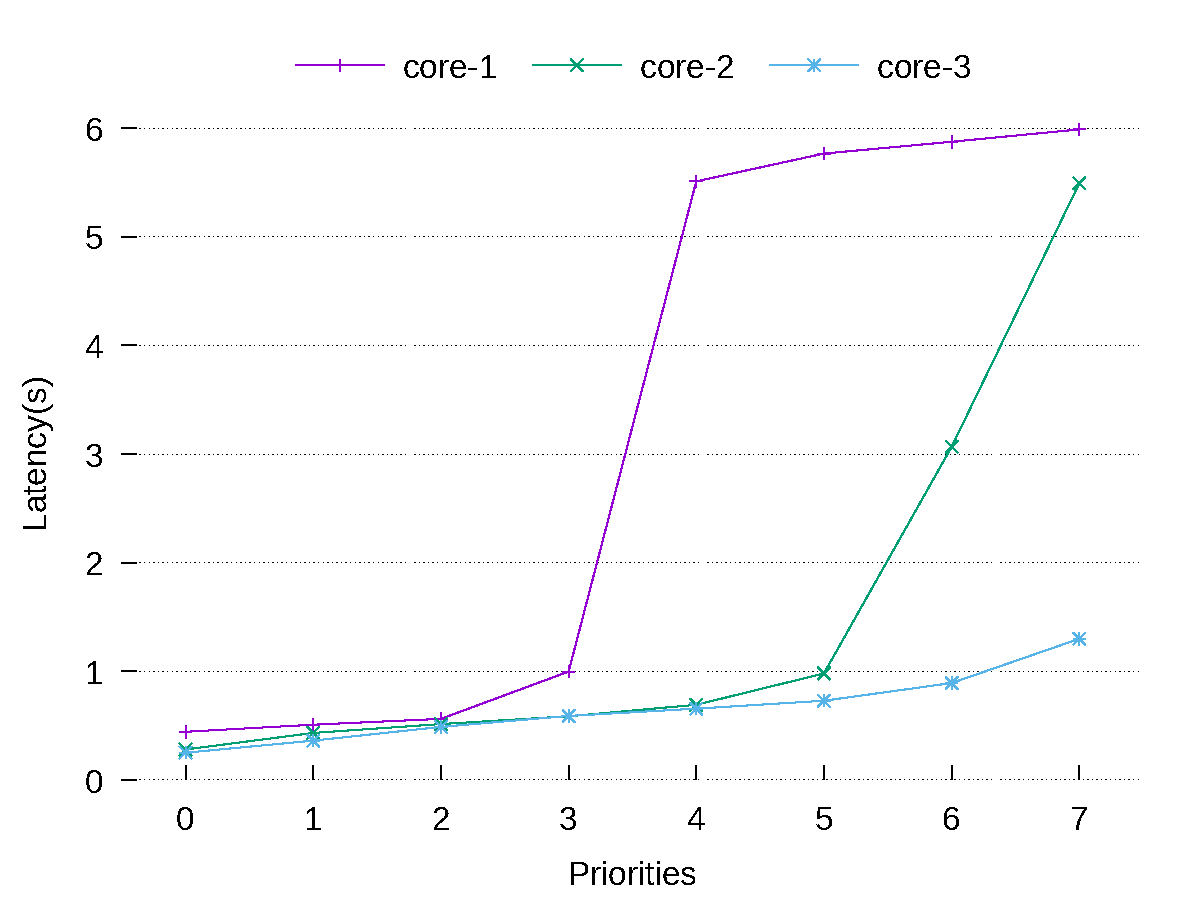
\includegraphics[width=\linewidth]{assets/prio-latency.pdf}
	}
	\caption{Throughput and message latency of different priority connections.}
	\label{fig:prio-throughput-latency}
	\vspace{-1.0em}
\end{figure}

In addition, we established 64 connections between the client and the server, evenly divided into 4 priorities, and analyzed the latency distribution for each priority connection. the final result is shown in Fig.~\ref{fig:prio-cores}. This is in line with the characteristics that the higher priority connections will be handled preferentially. High priority connections have concentrated latency distribution and low latency, while low priority connections have scattered latency and high latency. With the increase of resources, the latency of all priorities decreases and is concentrated.

\begin{figure}[ht]
    \centering
    \subcaptionbox{Core-2\label{subfig:prio-core2}}[0.49\linewidth]
    {
      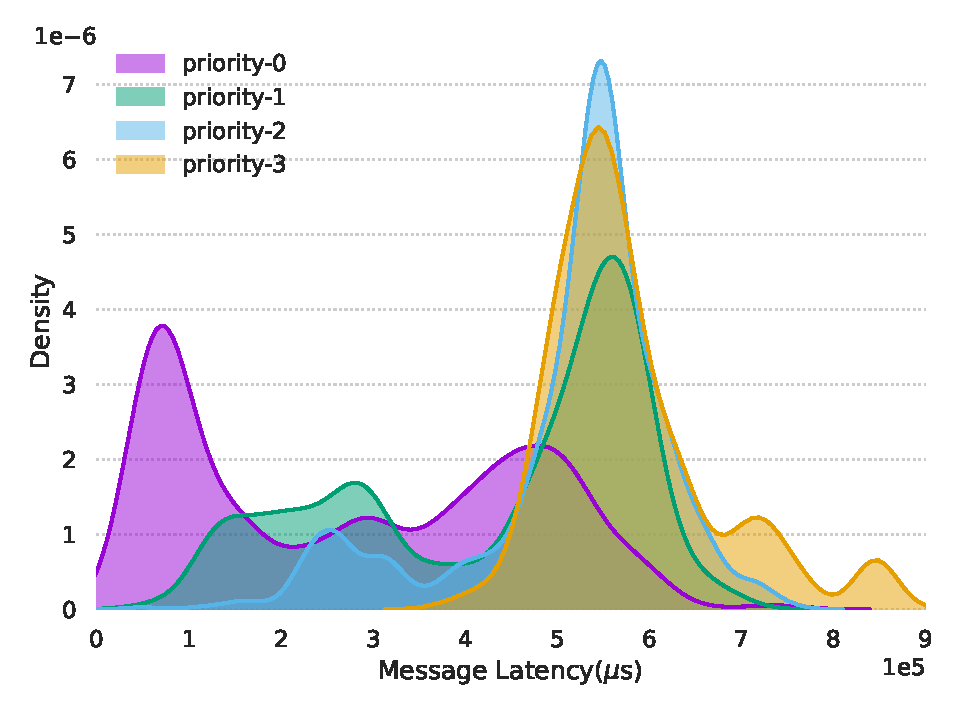
\includegraphics[width=\linewidth]{assets/prio-core2.pdf}
    }
    \subcaptionbox{Core-4\label{subfig:prio-core4}}[0.49\linewidth]
    {
      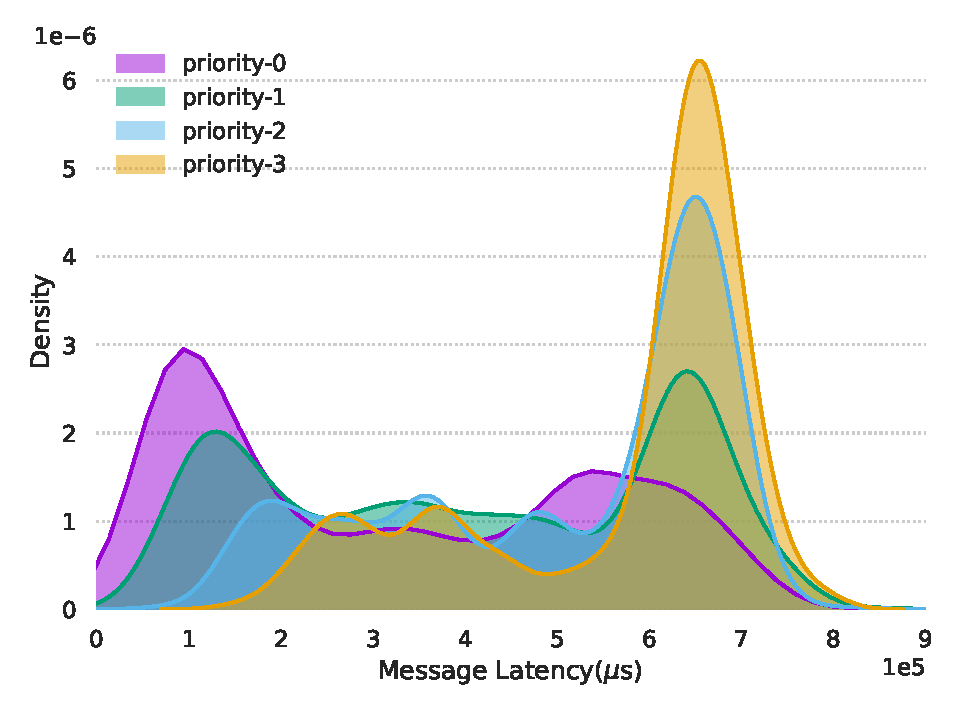
\includegraphics[width=\linewidth]{assets/prio-core4.pdf}
    }
    \caption{Latency distribution of different priority connections in different amount of cores.}
    \label{fig:prio-cores}
    \Description{Latency distribution of different priority connections in different amount of cores.}
\end{figure}

\section{Related Work}
\label{section: Related Work}

Coroutines are lightweight, have outstanding performance in context switches and are well-suited for the state-machine-based asynchronous event handling that I/O stacks commonly require. In recent years, a lot of research work has taken advantage of these advantages of coroutines.

Demikernel\cite{zhang_demikernel_2021} uses Rust coroutines to build their prototype system, avoiding the context switch overhead on the critical path of the IO stacks (approximately 12 cycles to complete the context switch). Besides, their TCP stack uses one coroutine per TCP connection for retransmissions, which keeps the relevant TCP state and removes the need for global TCP connection state management. They ultimately achieve microsecond latency.

Embassy\cite{embassy} is a generation framework of asynchronous driver for embedded environments based on Rust coroutines, achieves remarkable results in handling device interruptions. Compared with FreeRTOS implemented in C, it has achieved overwhelming advantages in terms of interrupt time consuming, thread time consuming, interrupt latency, etc.

\section{Conclusion}
\label{section: Conclusion}

This paper proposes COPS, a coroutine-based priority scheduling framework that can be perceived by the operating system. COPS make the kernel perceive the user-level coroutines by the priority bitmap mechanism and combines kernel coroutines with asynchronous I/O mechanisms. It is proved that COPS can help to develop highly concurrent applications, reduce the overhead of traditional multithreading model, and provide convenient asynchronous I/O mechanism and priority scheduling mechanism. Through the evaluation, we proved that the COPS framework can have the characteristics of high throughput and low latency in the construction of highly concurrent applications. Using the coroutine abstraction provided by COPS can increase throughput to 1.05x-3.93x than threads (KCUC vs KTUT). At the same time, the coroutine priority scheduling provided by COPS framework can cope with different needs well and ensure the reasonable allocation of system resources.

%%
%% The acknowledgments section is defined using the "acks" environment
%% (and NOT an unnumbered section). This ensures the proper
%% identification of the section in the article metadata, and the
%% consistent spelling of the heading.
\begin{acks}
To Robert, for the bagels and explaining CMYK and color spaces.
\end{acks}

% \balance

%%
%% The next two lines define the bibliography style to be used, and
%% the bibliography file.
\bibliographystyle{ACM-Reference-Format}
\bibliography{ref}

%%
%% If your work has an appendix, this is the place to put it.
\appendix


\end{document}
\endinput
%%
%% End of file `sample-sigconf.tex'.
